\section{Stream processing}
\large \textbf{Apache Kafka}\\
\normalsize
\textbf{Native stream processing}\\
From release v0.10, Kafka provides the Kafka Streams to support native stream processing \cite{kafkastreams}. This is a Java library built on top of Kafka producer and consumer. Users can use this library to implement and deploy stream processor which reads input records from Kafka and produces calculated results back to Kafka as a normal Java application. 

One of the main advantages of Kafka Streams is that users does not need to set up a separated cluster for stream processing. Normal Java application instance can be simply started anywhere to do the stream processing with Kafka. Moreover, since Kafka Streams is developed from normal Kafka client, it inherits the parallelism and failover concept of the Kafka consumer group. Multiple instances of a stream processor can be started for scalability. Each instance is assigned a set of partitions from the input topics. This also guarantees that records on the same partitions are processed by only one instance in the same order as when they are sent to Kafka. When the number of instances is changed due to failure or scaling up with more instances, the partition will be automatically rebalanced similar to the Kafka consumer group. Moreover, Kafka Streams also benefits from the features of idempotent producer and transaction of Kafka client. Therefore, exactly-once processing guarantee can be achieved with this library.

Kafka Streams library provides the Streams Domain Specific Language (DSL) which supports a rich set of functionalities. The DSL provides logical abstraction of Kafka topics as \emph{KStreams} and \emph{KTables}. A \emph{KStream} consists of all records in a Kafka topic while a \emph{KTable} only presents the latest values of each record key in the topic which is similar to a normal database table. The table representation can be very useful when doing lookup of the current state of an entity. 

The DSL supports a rich set of both stateless and stateful operations on top of its abstractions. There are many stateless operations such as filtering, mapping each record to a set of corresponding outputs. For stateful processing, the DSL support aggregating multiple records to extract result, joining \emph{KStreams} and \emph{KTables}, grouping records into window for processing. Users also have the flexibility to choose the semantics for the time boundaries of the windows such as event time (i.e. the time a record is actually generated at the source) or processing time (i.e. when the records are received by the stream processor). Users also have the possibility to choose different types of windows, control how the windows are advanced over time (Figure \ref{fig:windowtypes}).

\begin{figure}[h]
	\centering
	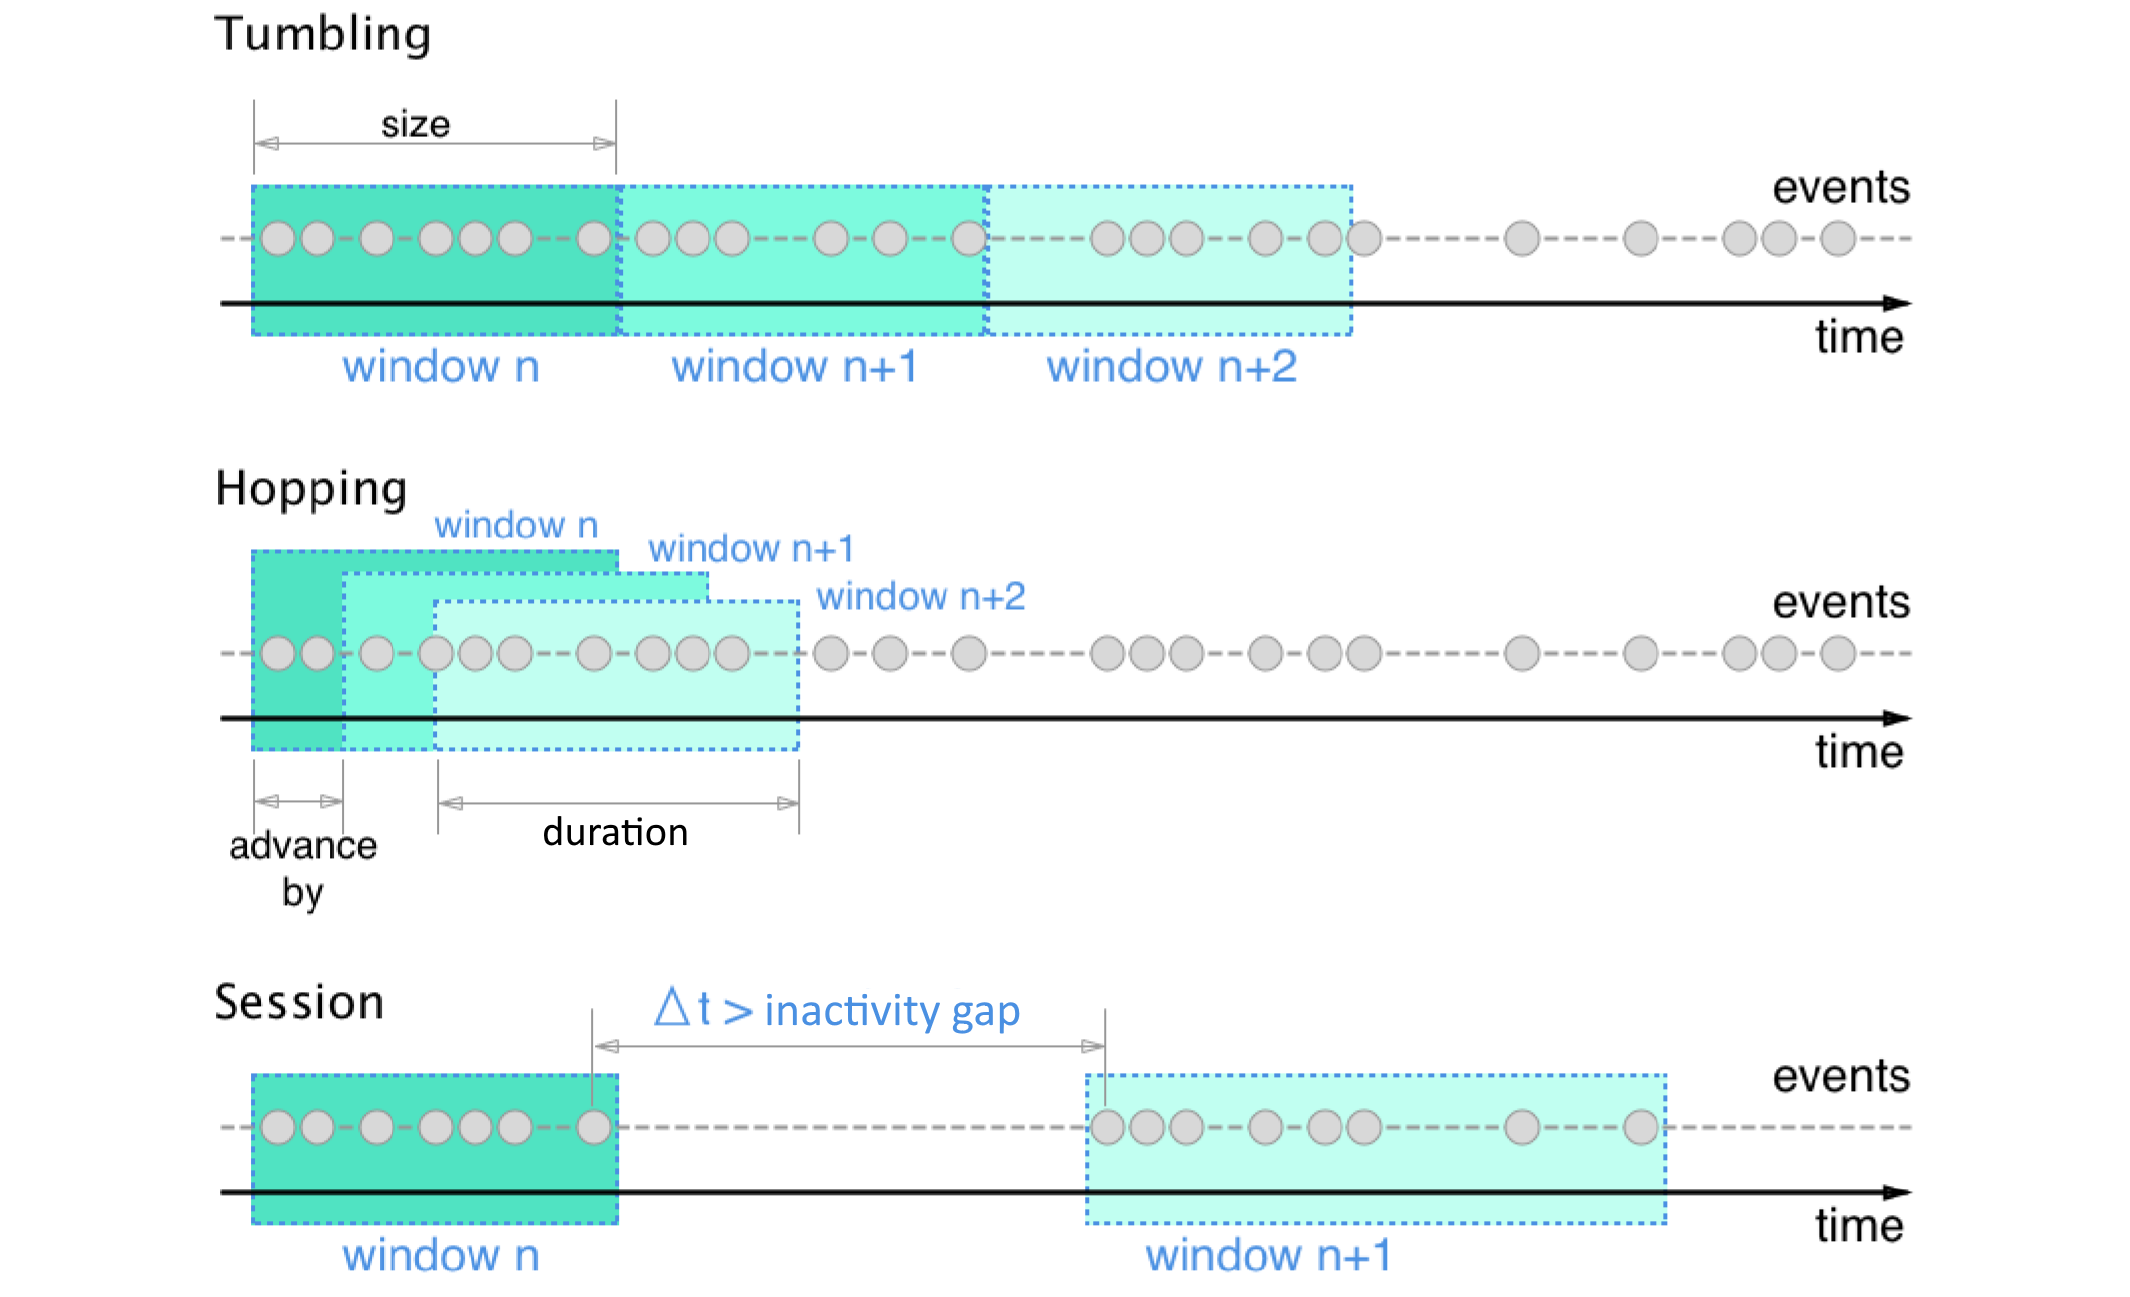
\includegraphics[width=\linewidth]{images/window-types.png}
	\caption{Supported window types for stream processing with Kafka Streams (taken from \cite{windowtypes}).}
	\label{fig:windowtypes}
\end{figure}

Each Kafka Streams application instance retains the current state of the stateful operations in a local state store. This has a number of advantages such as faster state query than remote storage, better isolation between the instances \cite{localstatestore}. Moreover, Kafka Streams also supports checkpointing the local state store to a Kafka topic for fault-tolerance which is managed completely transparent to users.

Apart from DSL, Kafka Streams also provides a lower-level Processor API. With this API, users have more flexibility to implement more sophisticated stateless and stateful operations which are not provided by the DSL. 

To sum up, Kafka Streams is a powerful tool to do stream processing on top of Kafka topics. Stream processors which are implemented using Kafka Streams not only benefit from various useful functions of the library, they can also integrate seamlessly with Kafka for scalability and fault-tolerance.





\large \textbf{Apache Pulsar}\\
\normalsize
\textbf{Native stream processing}\\
Apache Pulsar provides the Pulsar Functions for native stream processing \cite{pulsarfunction}. The concept of Pulsar Functions is similar to serverless function as a service (FaaS). Users can start a number of function workers on the Pulsar cluster. These workers can be run within the normal Pulsar brokers or they can be grouped into a separated cluster running on different host machines. 

Functions can be implemented using Java, Python or Go and deployed to the function workers. While deploying, the input topics and output topics of the function can be specified. Users can also configure the number of instances of the function to be run in parallel for scalability. Each instance is assigned to a function worker in the cluster where it is executed. Whenever a message arrives from one of the input topics, a function instance is triggered, and result is generated to the output topics. 

Internally, Pulsar Function uses Pulsar producer and consumer to read and write messages to Pulsar. By default, the internal Pulsar consumer uses Shared subscription mode to maximize the parallelism. In this case, messages on the input topics are distributed evenly across the instances of the function. Therefore, these messages can be processed out-of-order. To ensure that messages are handled in the right order, user must strictly enable that when deploying the function. If this is enabled, function will choose the Failover subscription mode for its consumer. In this way, each partition of a topic will be assigned to only one function instance and messages will be delivered and processed by the instance in the right order as when they are published to Pulsar.  

With Pulsar Functions, users can enforce stateless processing logic on each incoming message such as transforming, filtering, or routing to different output topics based on its content. The function also supports simple stateful stream processing. A function instance can aggregate input messages and persist the current state to Bookkeeper. Unlike local state store of Kafka Streams, the full state of a Pulsar function is maintained centrally in Bookkeeper. This state can be query directly by users using the REST API of the function worker or the command line tool provided by Pulsar.

Pulsar Functions also supports grouping messages into windows and generate corresponding results for each window. Nevertheless, this feature is still not properly documented and is also still unstable with unresolved issues \cite{pulsarfunctionissue}. More sophisticated stateful operation such as joining messages from two topics are not supported by Pulsar Functions. Moreover, Pulsar Functions currently does not support exactly-once processing guarantee since the transaction feature is still in technical review phase and not integrated into the function.

In summary, Pulsar Functions provides a simple and convenient way to quickly deploy functions to apply simple processing logic on the stream of messages on Pulsar. Because the functions run within the Pulsar cluster, no additional administrative tasks are required. Nevertheless, the available functionalities of Pulsar Functions are quite limited and cannot support more sophisticated streaming operations.

\large \textbf{NATS Streaming}\\
\normalsize
\textbf{Native stream processing}\\
NATS Streaming does not provide any tool for native stream processing. Users must implement the stream processing application from the ground up with NATS Streaming client or rely on external streaming processing framework such as Apache Spark or Apache Flink.
